\chapter{The Moon}\label{cmoon}
% !TEX root = ../Almagest.tex

\section{Lunar Ecliptic Longitude Model}
The orbit of the Moon around the Earth is strongly perturbed by the 
gravitational influence of the Sun. It follows that we cannot derive an accurate lunar longitude model
from Keplerian orbit theory alone. Instead, we shall employ a
greatly simplified version of modern lunar theory. According to such
theory, the time variation of the ecliptic longitude of the Moon is fairly
well represented by the following
formulae:\footnote {See  {\em Astronomical Algorithms}, J.~Meeus, (Willmann-Bell, Richmond VA, 1998).}
\begin{align}
\bar{\lambda} &=\bar{\lambda}_0  + n\,(t-t_0),\\[0.5ex]
M &= M_0 + \tilde{n}\,(t-t_0),\\[0.5ex]
\bar{F} &= \bar{F}_0 + \breve {n}\,(t-t_0),\\[0.5ex]
\tilde{D} &= \bar{\lambda} - \lambda_S,\\[0.5ex]
q_1 &= 2\,e\,\sin M + 1.2379\,e^2\,\sin 2M,\\[0.5ex]
q_2 &= 0.4052\,e\,\sin (2\tilde{D} - M),\\[0.5ex]
q_3 &= 0.2094\,e\,(\sin 2\tilde{D} - 0.0527\,\sin \tilde{D}),\\[0.5ex]
q_4 &= -0.0589\,e\,\sin M_S,\\[0.5ex]
q_5&= -0.0364\,e\,\sin 2 \bar{F},\\[0.5ex]
\lambda &= \bar{\lambda} + q_1+q_2+q_3+q_4+q_5.
\end{align}
Here, $\lambda_S$ and $M_S$ are the longitude and mean anomaly
of the Sun, respectively. Moreover, $e$, $\lambda$, $\bar{\lambda}$, $\bar{F}$,
and $q_i$ are the eccentricity, longitude, mean longitude, mean argument of latitude,
and $i$th anomaly of the Moon, respectively. The Moon's first anomaly
is due to the eccentricity of its orbit, and is very similar in form to that obtained from Keplerian orbit theory. (See Chapter~\ref{ckep}.) The
Moon's second, third, and fourth anomalies are knows as
{\em evection}, {\em variation}, and the {\em annual inequality}, respectively, and originate from
the perturbing influence of the Sun. Finally, the Moon's fifth anomaly is
called the {\em reduction to the ecliptic}, and is a consequence of the fact that the Moon's
orbit is slightly tilted with respect to the plane of the ecliptic.
Note that Ptolemy's lunar theory only takes the first two
lunar anomalies into account. 
The Moon's orbital elements---$e$, $n$, $\tilde{n}$, $\breve{n}$, 
$\bar{\lambda}_0$, $M_0$, and $F_0$---for the J2000 epoch are listed in Table~\ref{tmoon}. Note that the lunar perigee precesses in the
direction of the Moon's orbital motion at the rate of
$n-\tilde{n} = 0.11140^\circ $ per day, or $360^\circ$ in 8.85 years. This
very large precession rate (more than 2000 times the corresponding
precession rate for the Sun's apparent orbit) is another consequence of the strong
perturbing influence of the Sun on the Moon's orbit.
The previous formulae are capable of matching NASA ephemeris
data during the years 1995--2006 AD with a mean error of $5'$  and
a maximum error of $14'$. 

The ecliptic longitude of the Moon can be calculated with the aid of Tables~\ref{tmoonm} and \ref{tmoona}.
Table~\ref{tmoonm} allows the lunar mean longitude, $\bar{\lambda}$,  the mean anomaly, $M$, and  the mean argument of latitude, $\bar{F}$, to be determined as functions of time.
Table \ref{tmoona} specifies the lunar anomalies, $q_1$--$q_5$, as functions of their various arguments.

Incidentally, Table~\ref{tmoonm} contains essentially the same information as is contained in the ``Table of the Moon's mean motion'' (Κανόνες τῶν τῆς σελήνης μέσων κινήσεων) that
appears in Section~4 of Book~IV of the Almagest. Moreover, Table~\ref{tmoona} contains equivalent information to that contained in the ``Table of the whole lunar anomaly" (Κανόνιον τῆς καθόλου σεληνακῆς ἀνωμαλίας)
that appears in Section~8 of Book~V of the Almagest. 

\section{Determination of Lunar Ecliptic Longitude}
The procedure for using Tables~\ref{tmoon} and \ref{tmoona} to determine lunar longitude is as follows:
\begin{enumerate}
 
 \item Determine the fractional Julian day number, $t$, corresponding to the date and time
at which the Moon's ecliptic longitude is to be calculated with the aid of Tables~\ref{kt1}--\ref{kt3}. Form $\Delta t = t-t_0$, where $t_0=2\,451\,545.0$ is the epoch. 

\item Calculate the ecliptic longitude, $\lambda_S$, and the mean anomaly, $M_S$, of the
Sun using the procedure set out in Section~\ref{ssun}.

\item Enter Table~\ref{tmoonm} with the digit for each power of 10
in ${\Delta} t$ and take out the corresponding values of $\Delta\bar{\lambda}$, $\Delta M$,
and $\Delta\bar{F}$. If $\Delta t$ is negative then the 
values are minus those shown in the table.
The value of the mean longitude, $\bar{\lambda}$, is the
sum of all the $\Delta\bar{\lambda}$ values plus the value of $\bar{\lambda}$ at the epoch. Likewise, the value of the mean anomaly, $M$, is
the sum of all the $\Delta M$ values plus the value of $M$ at the epoch. Finally, the value of the mean argument of latitude, $\bar{F}$, is the
sum of all the $\Delta\bar{F}$ values plus the value of $\bar{F}$ at the epoch. 
Add as many multiples of $360^\circ$ to $\bar{\lambda}$, $M$, and $\bar{F}$
as is required to make them all fall in the range $0^\circ$ to $360^\circ$. 

\item Form $\tilde{D}=\bar{\lambda}-\lambda_S$. 

\item Form the five arguments $a_1=M$, $a_2=2\tilde{D} - M$, $a_3=\tilde{D}$, $a_4 = M_S$, $a_5=2\bar{F}$. Add as
many multiples of $360^\circ$ to the arguments as is required to make them all fall in the range
$0^\circ$ to $360^\circ$. Round each argument to the nearest degree.

\item Enter Table~\ref{tmoona} with the value of each of the five arguments $a_1$--$a_5$ and take out the
value of each of the five corresponding  anomalies $q_1$--$q_5$. It is necessary to interpolate if the arguments are odd.

\item The Moon's ecliptic longitude is given by $\lambda=\bar{\lambda} + q_1+q_2+q_3+q_4+q_5$.
If necessary, convert $\lambda$ into an angle in the range $0^\circ$ to $360^\circ$. 
The decimal fraction can be converted into arc minutes
using Table~\ref{lt6a}. Round to the nearest arc minute. 
\end{enumerate}

Two examples of the use of the procedure that has just been described are given in the following section.

\section{Example Lunar Longitude Calculations}\label{exllat}
\noindent {\em Example 1}: May 5, 2005 AD, 00:00 UT:\\
~\\
From Section~\ref{ssun}, $t-t_0=1950.5$ JD, $\lambda_S = 44.602^\circ$, and $M_S= 120.001^\circ$. 
Making use of Table~\ref{tmoonm}, we find:\\
\begin{tabular}{rrrr}
&&&\\
$t$(JD) & $ \bar{\lambda}(^\circ)$ & $M(^\circ)$ & $\bar{F}(^\circ)$\\[-2ex]
&&&\\
$+1\,000$ & $216.396$ & $104.993$ & $269.350$\\
$+900$ & $338.757$ & $238.494$ & $26.415$\\
$+50$ & $298.820$ & $293.250$ & $301.468$\\
$+.5$ & $6.588$ & $6.532$ & $6.615$\\
Epoch & $218.322$ & $134.916$ & $93.284$\\\cline{2-4}
&$1078.883$ & $778.185$ & $697.132$\\\cline{2-4}
Modulus & $358.883$ & $58.185$ &$337.132$\\ 
&&&\\
\end{tabular}\\
It follows that 
$$
\tilde{D}=\bar{\lambda}-\lambda_S = 358.883-44.602 = 314.281^\circ.
$$
Thus, 
$$
a_1=M\simeq 58^\circ,~~~a_2=2\tilde{D}-M = 2\times 314.281-58.185=570.377\simeq 210^\circ,
$$ 
$$
a_3=\tilde{D}\simeq 314^\circ,~~~a_4 = M_S\simeq 120^\circ,
$$ 
$$
a_5=2\bar{F} = 2\times 337.132=674.264\simeq 314^\circ.
$$
Table~\ref{tmoona} yields $$
q_1(a_1)=5.525^\circ,~~q_2(a_2)= -0.637^\circ,~~q_3(a_3) = -0.633^\circ,
$$
$$q_4(a_4)=-0.160^\circ,~~q_5(a_5)= 0.082^\circ.
$$
 Hence,
$$
\lambda = \bar{\lambda} + q_1+q_2+q_3+q_4+q_5=358.883+5.525-0.637-0.633-0.160+0.082=
363.060^\circ,
$$
or 
$$
\lambda =3.060\simeq 3^\circ 04'.
$$
Thus, the ecliptic longitude of the Moon at 00:00 UT on May 5, 2005 AD was 3AR04.

~\\
\noindent {\em Example 2}: December 25, 1800 AD, 00:00 UT:\\
~\\
From Section~\ref{ssun}, $t-t_0=-72\,690.5$ JD, $\lambda_S = 273.055^\circ$, and $M_S= 353.814^\circ$. 
Making use of Table~\ref{tmoonm}, we find:\\
\begin{tabular}{rrrr}
&&&\\
$t$(JD) & $ \bar{\lambda}(^\circ)$ & $M(^\circ)$ & $\bar{F}(^\circ)$\\[-2ex]
&&&\\
$-70\,000 $& $-27.752$ & $-149.506$ & $-134.519$\\
$-2\,000$ & $-72.793$ & $-209.986$ & $-178.701$\\
$-600$ & $-345.838$ & $-278.996$ & $-17.610$\\
$-90$ & $-105.876$ & $-95.849$ & $-110.642$\\
$-.5$ & $-6.588$ & $-6.532$ & $-6.615$\\
Epoch & $218.322$ & $134.916$ & $93.284$\\\cline{2-4}
&$-340.525$ & $-605.953$ & $-354.803$\\\cline{2-4}
Modulus & $19.475$ & $114.047$ &$5.197$\\ 
&&&\\
\end{tabular}\\
It follows that $$
\tilde{D}=\bar{\lambda}-\lambda_S = 19.475-273.055 = -253.580^\circ.
$$
Thus, 
$$
a_1=M\simeq 114^\circ,~~~a_2=2\tilde{D}-M = -2\times 253.580-114.047=-621.207 \simeq 99^\circ,
$$ 
$$
a_3=\tilde{D}\simeq 106^\circ,~~~a_4 = M_S\simeq 354^\circ,
$$ 
$$
a_5=2\bar{F} = 2\times 5.197=10.394\simeq 10^\circ.
$$
Table~\ref{tmoona} yields $$
q_1(a_1)=5.586^\circ,~~q_2(a_2)= 1.259^\circ,~~q_3(a_3) = -0.382^\circ,
$$
$$q_4(a_4)=0.019^\circ,~~q_5(a_5)= -0.020^\circ.
$$
 Hence,
$$
\lambda = \bar{\lambda} + q_1+q_2+q_3+q_4+q_5=19.475+5.586+1.259-0.382+0.019-0.020=
25.937^\circ,
$$
or 
$$
\lambda =25.937\simeq 25^\circ 56'.
$$
Thus, the ecliptic longitude of the Moon at 00:00 UT on December 25, 1800 AD was 25AR56.

\begin{figure}[h]
\centerline{\includegraphics[height=3.5in]{epsfiles/Node.eps}}
\caption{The orbit of the Moon about the Earth.  Here, $G$, $L$, $N$, $N'$,   $\Omega$, $F$, and $\Upsilon$
represent the Earth, the Moon, the ascending node, the descending node, the longitude of the ascending node, the argument of latitude, and the vernal equinox, respectively. The view is from northern ecliptic pole. The Moon orbits counterclockwise.}\label{fmoon}
\end{figure}

\section{Lunar Ecliptic Latitude Model}
A model of the Moon's ecliptic latitude is needed in order to predict the
occurrence of solar and lunar eclipses. Figure~\ref{fmoon} shows the
Moon's orbit about the Earth. The plane of this orbit is fixed, but slightly tilted with
respect to the plane of the ecliptic (that is, the plane of the Sun's
apparent orbit about the Earth). Let the two planes intersect along the
line of nodes, $NGN'$. Here, $N$ is the point at which the orbit crosses the
ecliptic plane from south to north (in the direction of the Moon's orbital
motion), and is termed the {\em ascending node}. Likewise, $N'$ is the
point at which the orbit crosses the ecliptic plane from north to south,
and is called the {\em descending node}. Incidentally, the line of nodes must pass through point $G$, because the Earth is common to the ecliptic plane and the plane of the lunar orbit.
The angle, $\Omega$, subtended between
 the radius vector $G\Upsilon$, connecting the Earth to the vernal equinox,
and the line $GN$, is known as the {\em longitude of the ascending node}. Note, incidentally, that
the ascending node precesses in the opposite direction to the Moon's orbital motion
at the rate  $\breve{n}-n = 5.2954\times 10^{-2}\,^\circ$ per day, or $360^\circ$ in 18.6 years. 
This unusually large precession rate is another consequence of the Sun's strong perturbing influence on the
Moon's orbit.
Let the line $MGM'$ lie in the plane
of the Moon's orbit such that it is perpendicular to $NGN'$.
The inclination, $i$,  of the Moon's orbital plane is the angle
that $GM$ subtends with its projection onto the ecliptic plane. Likewise, the
Moon's ecliptic longitude, $\beta$, is the angle that $GL$ subtends with its
projection onto the ecliptic plane.
Simple geometry
yields $\sin\beta = \sin i\,\sin F$, where $F$ is the angle
between $GN$ and $GL$. This angle is termed the {\em argument of latitude.} 
Now, it is easily seen that $F \simeq \lambda-\Omega$, where $\lambda$
is the Moon's ecliptic longitude (that is, the angle subtended
between  $G\Upsilon$ and $GL$). Here, we are assuming that the orbital
inclination $i$ is relatively
small. The {\em mean argument of latitude}\/ is defined $\bar{F} = \bar{\lambda}-\Omega$. 
 Hence, our model for the Moon's ecliptic latitude becomes
\begin{align}
F &=\bar{F}+q_1+q_2+q_3+q_4+q_5,\\[0.5ex]
\sin\beta &= \sin i\,\sin F.\label{emoonlat}
\end{align}
The value of the lunar orbital inclination, $i$,  for the
J2000 epoch is specified in Table~\ref{tmoon}. The previous model is capable of
matching NASA ephemeris data during the years 1995-2006 AD with
a mean error of $6'$, and a maximum error of $11'$.

\section{Determination of Lunar Ecliptic Latitude}
The ecliptic latitude of the Moon can be calculated with the aid of Table~\ref{tmoonb}. The procedure for using this table is as follows:
\begin{enumerate}

 \item Determine the fractional Julian day number, $t$, corresponding to the date and time
at which the Moon's ecliptic latitude is to be calculated with the aid of Tables~\ref{kt1}--\ref{kt3}. Form $\Delta t = t-t_0$, where $t_0=2\,451\,545.0$ is the epoch. 

\item Calculate the lunar mean argument of latitude, $\bar{F}$, 
and the five lunar anomalies, $q_1$--$q_5$, using the procedure outlined earlier in this 
section.

\item Form the argument $F = \bar{F}+q_1+q_2+q_3+q_4+q_5$. Add as many multiples of $360^\circ$ to $F$ as is required to make it fall in the range
$0^\circ$ to $360^\circ$. Round $F$ to the nearest degree.

\item Enter Table~\ref{tmoonb} with the value of $F$
and take out the lunar ecliptic latitude, $\beta$. It is necessary to
interpolate if $F$ is odd.
\end{enumerate}

Two examples of the use of the procedure that has just been described are given in the following section.

\section{Example Lunar Latitude Calculations}
\noindent {\em Example 1}: May 5, 2005 AD, 00:00 UT:\\
~\\
We have already seen in Section~\ref{exllat} that at 00:00 UT on May 5, 2005 AD
the lunar mean argument of latitude, and
the lunar anomalies, were $\bar{F}=337.132^\circ$, and
$q_1=5.525^\circ$, $q_2=-0.637^\circ$, $q_3=-0.633^\circ$, $q_4=-0.160^\circ$,
and $q_5=0.082^\circ$, respectively. Hence, $F=\bar{F}+q_1+q_2+q_3+q_4+q_5
=337.132+5.525-0.637-0.633-0.160+0.082\simeq 341^\circ$. Thus, according to Table~\ref{tmoonb}, the ecliptic latitude
of the Moon at  00:00 UT on May 5, 2005 AD was $-1.678^\circ\simeq -1^\circ 41'$.

~\\
\noindent {\em Example 2}: December 25, 1800 AD, 00:00 UT:\\
~\\
We have already seen in Section~\ref{exllat} that at 00:00 UT on December 25, 1800 AD
the lunar mean argument of latitude, and
the lunar anomalies, were $\bar{F}=5.197^\circ$, and
$q_1=5.586^\circ$, $q_2=1.259^\circ$, $q_3=-0.382^\circ$, $q_4=-0.019^\circ$,
and $q_5=-0.020^\circ$, respectively. Hence, $F=\bar{F}+q_1+q_2+q_3+q_4+q_5
=5.197+5.586+1.259-0.382-0.019-0.020\simeq 12^\circ$. Thus, according to Table~\ref{tmoonb}, the ecliptic latitude
of the Moon at  00:00 UT on December 25, 1800 AD was $+1.072^\circ\simeq +1^\circ 04'$.

\section{Length of Month}
A {\em sidereal month}\/ is the mean period of time between successive passages of the Moon through the vernal equinox, and is
$360/n= 360/13.17639646=27.326$ days in length, where $n$ comes from Table~\ref{tmoon}. A {\em synodic month}\/ is the mean period of time between successive new moons, or
successive full moons, and is $360/(n-n_S)= 360/(13.17639646-0.98564735)=29.531$ days in length, where $n_S$ (which is the mean motion of the Sun) comes from Table~\ref{lt4}. 
An {\em anomalistic month}\/ is the mean period of time between successive passages of the Moon through its perigee, and is $360/\tilde{n}=360/13.06499295=27.555$ days
in length, where $\tilde{n}$ comes from Table~\ref{tmoon}. Finally, a {\em draconic month}\/ is the mean period of time between successive passages of the Moon
through its ascending node, and is $360/\breve{n} =360/13.22935027 = 27.212$ days in length, where $\breve{n}$ comes from Table~\ref{tmoon}. 

\begin{figure}
\centerline{\includegraphics[height=3in]{epsfiles/parallax.eps}}
\caption{The Moon, $L$, as viewed by a hypothetical observer, $C$,
at the center of the Earth,  and a real observer, $X$, on the
surface of the Earth.}\label{fpara}
\end{figure}

\section{Lunar Parallax}\label{spara}
Now, it turns out that the Moon is sufficiently close to the Earth that its position in the sky is
significantly modified by {\em parallax}. All of our previous analysis
applies to a hypothetical observer situated at the center of the Earth.
Consider a real observer situated on the Earth's surface. It can
be seen from Figure~\ref{fpara} that the altitude of the Moon is
$a'$ for the real observer, and $a$ for the hypothetical observer. Simple
trigonometry reveals that $a' = a-\delta a$, which implies that the real
observer sees the Moon at a  lower altitude than the hypothetical observer.
Let $R$ be the radius of the Earth, and $r$ the distance from the center
of the Earth to the Moon. More simple trigonometry yields
\begin{equation}
\sin \delta a = \frac{R}{r}\,\cos a'.
\end{equation}
Let us assume that the Moon's orbit is elliptical to first order in its
eccentricity. It follows, from Chapter~\ref{ckep}, that
\begin{equation}
r \simeq a_M\,(1 - e\,\cos M),
\end{equation}
where $a_M$, $e$, and $M$ are major radius, eccentricity, and mean
anomaly of the lunar orbit, respectively. Assuming that $\delta a$ is small, we
obtain
\begin{equation}\label{ea112}
\delta a \simeq \delta a_0\,\cos a\,(1+e\,\cos M),
\end{equation}
where $\delta a_0 = R/a_M = 0.016574=56.98'$ (because $R=6371$ km and $a_M=384\,399$ km). 

According to Equation~(\ref{ea112}), lunar parallax can be written in the form
\begin{equation}
\delta a = \delta (a)\,[1+\zeta (M)],
\end{equation}
where $a$, $a-\delta a$, and $M$ are the Moon's geocentric altitude (that is, the altitude seen from the center of the Earth), true
altitude, and mean anomaly, respectively. The functions $\delta(a)=\delta a_0\,\cos a$ and
$\zeta (M)= e\,\cos M$ are tabulated in Table~\ref{tmoonc}. It can be seen from the
table that lunar parallax increases with decreasing lunar altitude, reaching a maximum value of about $57'$ when the Moon is close to the horizon.
For example, if $a=44^\circ 00'$ and $M=100^\circ$ then Table~\ref{tmoonc}
yields $\delta = 40.988'$ and $\zeta =- 0.00953$. Hence, $\delta a = 40.988\,(1-0.00953) \simeq 41'$, and the true altitude of the Moon becomes
$43^\circ 19'$. 

Incidentally, the information contained in Table~\ref{tmoonc} is equivalent to that contained in the ``Parallax table" (Κανὼν παραλλακτικός) that appears in Section~18 of
Book~V of the Almagest. Moreover, in Section~15 of the same book, Ptolemy uses the measured lunar parallax to determine the distance of the Moon from
the Earth. Ptolemy finds that the Moon is $59$ Earth radii from the center of the Earth. (The correct Earth-Moon distance  is $60.33$ Earth radii.) Furthermore, in Section~16
of the same book, Ptolemy uses his Earth-Moon distance, in combination with the apparent size of the Moon in the sky, to estimate that the Earth's radius is $3.4$ times
that of the Moon. (The correct answer is that the Earth's radius is $3.67$ times that of the Moon.)

\begin{figure}
\centerline{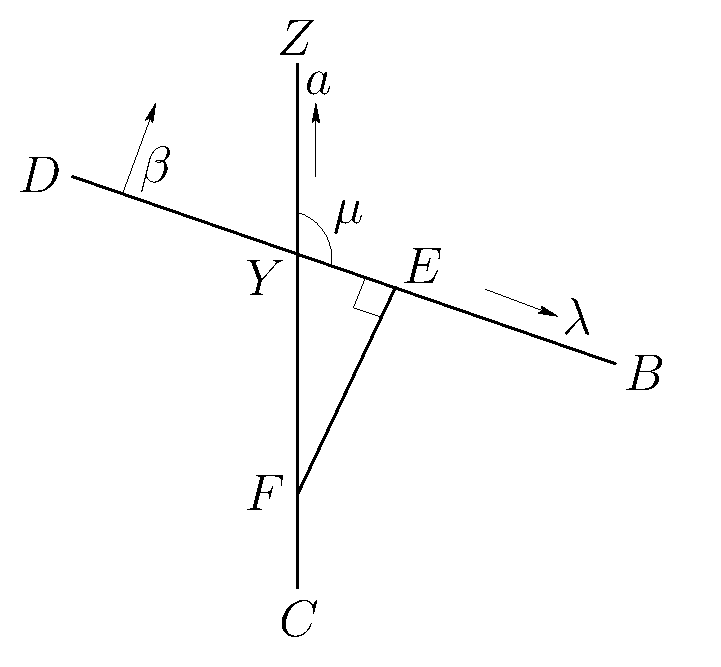
\includegraphics[height=3in]{epsfiles/para.eps}}
\caption{ Parallactic shifts in the Moon's ecliptic longitude and latitude.}\label{fpara1}
\end{figure}

It now remains to investigate how parallax affects the Moon's ecliptic
longitude and latitude. Figure~\ref{fpara1} shows a detail of Figure~\ref{f11}. Point $Y$ is the Moon's geocentric position on the celestial sphere. $DB$ is a line passing through this point
that is parallel to the local ecliptic circle, whereas $ZC$ is a small section of an
altitude circle passing through $Y$. The angle subtended between the ecliptic and the altitude circle is the parallactic angle, $\mu$. Let $F$ be the true position of the Moon.
It follows that $\delta a = YF$. The changes in the Moon's ecliptic longitude
and latitude are $\delta\lambda = YE$ and  $-\delta\beta = EF$, respectively. Here, we are considering the case where   increasing 
altitude corresponds to  increasing ecliptic latitude.
Assuming that the arcs $\delta a$, $\delta\lambda$, and $\delta\beta$ are
all fairly small, the triangle $YEF$ can be treated as a plane triangle.
Hence, we obtain
\begin{align}\label{epara1}
\delta\lambda &= - \delta a\,\cos\mu,\\[0.5ex]
\delta\beta &= - \delta a\,\sin\mu.\label{epara2}
\end{align}
As is easily demonstrated, the previous formulae also apply to the case in which increasing  altitude corresponds
to  decreasing  ecliptic latitude.

For example, consider a day on which the geocentric ecliptic longitude  and mean anomaly
of the Moon are $\lambda=210^\circ$ (that is, 00SC00) and $M=90^\circ$, respectively. Suppose that the Moon is
viewed from an observation site located  at terrestrial latitude $+10^\circ$. 
The ``Scorpio'' entry in Table~\ref{tscorp} gives the Moon's geocentric altitude, $a$, as a function of time, as well as the
value of the parallactic angle $\mu$. Making use of this data,
in combination with Table~\ref{tmoonc} and Equations~(\ref{epara1}) and (\ref{epara2}), we can calculate the parallax-induced changes in the Moon's ecliptic
longitude and latitude as it transits the sky. 
Data from such a calculation is given in the following table. The first column specifies
time since the  Moon's upper transit (thus, $t=+1$ hrs.\ means one hour after  the
upper transit), the second column gives the Moon's geocentric altitude, the third column the parallactic angle, 
the
fourth column the decrease in the Moon's real altitude due to parallax, and the fifth and
sixth columns the parallax-induced changes in its ecliptic longitude and latitude, respectively. 
It can be seen that parallax causes the Moon's apparent location
 to shift by almost $2^\circ$ relative to the fixed stars as it transits the sky. Note that the
previous calculation is somewhat inaccurate because it does not take into account the Moon's motion along the
ecliptic (which can easily amount to $6^\circ$ during the course of a night).
However, the calculation does illustrate how the data contained in
Tables~\ref{ltxx}--\ref{ltyy}, in combination with the data in Table~\ref{tmoonc}, permits the parallax-induced shift in the Moon's ecliptic position
to be calculated for a wide range of different lunar phases,
observation sites, and observation times.

~\\
\begin{tabular}{r|ccccc}\centering
$t$ (hrs.) & $a $ & $\mu$ & $\delta a $ & $\delta\lambda $ & $\delta\beta$\\\hline
&&&\\[-1.75ex]
$-5.52$ & $00^\circ 00'$  & $190^\circ 22'$ & $57'$ &$+56'$ & $+10'$\\
$-5.00$ & $12^\circ 26'$ & $187^\circ 30'$ & $56'$ & $+55'$ & $+07'$\\
$-4.00$ & $26^\circ  37'$ & $183^\circ 07'$ & $51'$ & $+51'$&$+03'$\\
$-3.00$ & $40^\circ 23'$ & $176^\circ 40'$ & $43'$ &$+43'$ & $-03'$\\
$-2.00$ & $53^\circ 15'$ & $165^\circ 58'$ & $34'$ & $+33'$&$-08'$\\
$-1.00$ & $63^\circ 52'$ & $145^\circ 55'$ & $25'$ & $+21'$&$-14'$\\
$+0.00$ & $68^\circ 32'$ & $110^\circ 34'$ & $21'$ & $+07'$ & $-20'$\\
$+1.00$ & $63^\circ 52'$ & $075^\circ 13'$ & $25'$ & $-06'$&$-24'$\\
$+2.00$ & $53^\circ 15'$ & $055^\circ 11'$ & $34'$ & $-19'$&$-28'$\\
$+3.00$ & $40^\circ 23'$ & $044^\circ 29'$ & $43'$ & $-31'$&$-30'$\\
$+4.00$ & $26^\circ 37'$ & $038^\circ01'$ & $51'$ & $-40'$&$-31'$\\
$+5.00$& $12^\circ 26'$ & $033^\circ 39'$ & $56'$ & $- 46'$&$-31'$\\
$+5.52$ & $00^\circ 00'$ & $030^\circ 47'$ & $57'$ & $-49'$&$-29'$\\
\end{tabular}\\
~\\~\\~\\

\newpage
\begin{table}[h]
\begin{tabular}{cccccccc}
$e$ & $n(^\circ/{\rm day})$ &  $\tilde{n}(^\circ/{\rm day})$  & $\breve{n}(^\circ/{\rm day})$
& $ \bar{\lambda}_0(^\circ)$ & $M_0(^\circ)$ & $ F_0(^\circ)$ & $i(^\circ)$ \\\hline
0.054881 & 13.17639646 & 13.06499295& $13.22935027$ &
218.322 & 134.916 & 93.284& 5.161\\
\end{tabular}
\caption{Orbital elements of the Moon for the J2000 epoch (that is, 12:00 UT, January 1, 2000 AD,
which corresponds to $t_0 = 2\,451\,545.0$ JD).}\label{tmoon}
\end{table}

\clearpage
\begin{table}
\centering
\begin{tabular}{rrrr|rrrr}
$\Delta t$(JD)& $\Delta\bar{\lambda}(^\circ)$ &  $\Delta M(^\circ)$ & $\Delta \bar{F}(^\circ)$& $\Delta t$(JD) & $\Delta\bar{\lambda}(^\circ)$ & $\Delta M(^\circ)$ 
&$\Delta \bar{F}(^\circ)$\\ \hline
&&&&&&&\\[-1.75ex]
10\,000 &   3.965 & 329.930 & 173.503 & 1\,000 & 216.396 & 104.993 & 269.350\\
20\,000 &   7.929 & 299.859 & 347.005 & 2\,000 &  72.793 & 209.986 & 178.701\\
30\,000 &  11.894 & 269.788 & 160.508 & 3\,000 & 289.189 & 314.979 &  88.051\\
40\,000 &  15.858 & 239.718 & 334.011 & 4\,000 & 145.586 &  59.972 & 357.401\\
50\,000 &  19.823 & 209.648 & 147.513 & 5\,000 &   1.982 & 164.965 & 266.751\\
60\,000 &  23.788 & 179.577 & 321.016 & 6\,000 & 218.379 & 269.958 & 176.102\\
70\,000 &  27.752 & 149.506 & 134.519 & 7\,000 &  74.775 &  14.951 &  85.452\\
80\,000 &  31.717 & 119.436 & 308.022 & 8\,000 & 291.172 & 119.944 & 354.802\\
90\,000 &  35.681 &  89.366 & 121.524 & 9\,000 & 147.568 & 224.937 & 264.152\\
&&&&&&&\\
100 & 237.640 & 226.499 & 242.935 & 10 & 131.764 & 130.650 & 132.294\\
200 & 115.279 &  92.999 & 125.870 & 20 & 263.528 & 261.300 & 264.587\\
300 & 352.919 & 319.498 &   8.805 & 30 &  35.292 &  31.950 &  36.881\\
400 & 230.559 & 185.997 & 251.740 & 40 & 167.056 & 162.600 & 169.174\\
500 & 108.198 &  52.496 & 134.675 & 50 & 298.820 & 293.250 & 301.468\\
600 & 345.838 & 278.996 &  17.610 & 60 &  70.584 &  63.900 &  73.761\\
700 & 223.478 & 145.495 & 260.545 & 70 & 202.348 & 194.550 & 206.055\\
800 & 101.117 &  11.994 & 143.480 & 80 & 334.112 & 325.199 & 338.348\\
900 & 338.757 & 238.494 &  26.415 & 90 & 105.876 &  95.849 & 110.642\\
&&&&&&&\\
1 &  13.176 &  13.065 &  13.229 & 0.1 &   1.318 &   1.306 &   1.323\\
2 &  26.353 &  26.130 &  26.459 & 0.2 &   2.635 &   2.613 &   2.646\\
3 &  39.529 &  39.195 &  39.688 & 0.3 &   3.953 &   3.919 &   3.969\\
4 &  52.706 &  52.260 &  52.917 & 0.4 &   5.271 &   5.226 &   5.292\\
5 &  65.882 &  65.325 &  66.147 & 0.5 &   6.588 &   6.532 &   6.615\\
6 &  79.058 &  78.390 &  79.376 & 0.6 &   7.906 &   7.839 &   7.938\\
7 &  92.235 &  91.455 &  92.605 & 0.7 &   9.223 &   9.145 &   9.261\\
8 & 105.411 & 104.520 & 105.835 & 0.8 &  10.541 &  10.452 &  10.583\\
9 & 118.588 & 117.585 & 119.064 & 0.9 &  11.859 &  11.758 &  11.906\\
\end{tabular}
\caption{Mean motion of the Moon.  Here, $\Delta t = t-t_0$, $\Delta\bar{\lambda} = \bar{\lambda}-\bar{\lambda}_0$, $\Delta M = M - M_0$, and $\Delta\bar{F}= \bar{F}-\bar{F}_0$. 
At epoch  ($t_0 = 2\,451\,545.0$ JD), $\bar{\lambda}_0 = 218.322^\circ$, $M_0 = 134.916^\circ$,
and $\bar{F}_0 = 93.284^\circ$.}\label{tmoonm}
\end{table}

\newpage
\begin{table}\centering
\small{ \begin{tabular}{rrrrrr|rrrrrr}
Arg. ($^\circ$) & $q_1(^\circ)$  & $q_2(^\circ)$ & $q_3(^\circ)$ & $q_4(^\circ)$  & $q_5(^\circ)$ &
Arg. ($^\circ$) & $q_1(^\circ)$  & $q_2(^\circ)$ & $q_3(^\circ)$ & $q_4(^\circ)$  & $q_5(^\circ)$  \\\hline
&&&&&&&&&&&\\[-1.75ex]
000(360) & $+0.000$ & $+0.000$ & $+0.000$ & $-0.000$ & $-0.000$ & 090(270) & $+6.289$ & $+1.274$ & $-0.035$ & $-0.185$ & $-0.114$\\
002(358) & $+0.234$ & $+0.044$ & $+0.045$ & $-0.006$ & $-0.004$ & 092(268) & $+6.270$ & $+1.273$ & $-0.081$ & $-0.185$ & $-0.114$\\
004(356) & $+0.468$ & $+0.089$ & $+0.089$ & $-0.013$ & $-0.008$ & 094(266) & $+6.244$ & $+1.271$ & $-0.126$ & $-0.185$ & $-0.114$\\
006(354) & $+0.702$ & $+0.133$ & $+0.133$ & $-0.019$ & $-0.012$ & 096(264) & $+6.210$ & $+1.267$ & $-0.171$ & $-0.184$ & $-0.114$\\
008(352) & $+0.934$ & $+0.177$ & $+0.177$ & $-0.026$ & $-0.016$ & 098(262) & $+6.169$ & $+1.262$ & $-0.216$ & $-0.183$ & $-0.113$\\
010(350) & $+1.165$ & $+0.221$ & $+0.219$ & $-0.032$ & $-0.020$ & 100(260) & $+6.120$ & $+1.255$ & $-0.259$ & $-0.182$ & $-0.113$\\
012(348) & $+1.394$ & $+0.265$ & $+0.261$ & $-0.039$ & $-0.024$ & 102(258) & $+6.065$ & $+1.246$ & $-0.302$ & $-0.181$ & $-0.112$\\
014(346) & $+1.622$ & $+0.308$ & $+0.301$ & $-0.045$ & $-0.028$ & 104(256) & $+6.002$ & $+1.236$ & $-0.343$ & $-0.180$ & $-0.111$\\
016(344) & $+1.847$ & $+0.351$ & $+0.339$ & $-0.051$ & $-0.032$ & 106(254) & $+5.932$ & $+1.225$ & $-0.382$ & $-0.178$ & $-0.110$\\
018(342) & $+2.069$ & $+0.394$ & $+0.376$ & $-0.057$ & $-0.035$ & 108(252) & $+5.856$ & $+1.212$ & $-0.420$ & $-0.176$ & $-0.109$\\
020(340) & $+2.288$ & $+0.436$ & $+0.411$ & $-0.063$ & $-0.039$ & 110(250) & $+5.772$ & $+1.197$ & $-0.456$ & $-0.174$ & $-0.108$\\
022(338) & $+2.504$ & $+0.477$ & $+0.444$ & $-0.069$ & $-0.043$ & 112(248) & $+5.683$ & $+1.181$ & $-0.490$ & $-0.172$ & $-0.106$\\
024(336) & $+2.717$ & $+0.518$ & $+0.475$ & $-0.075$ & $-0.047$ & 114(246) & $+5.586$ & $+1.164$ & $-0.521$ & $-0.169$ & $-0.105$\\
026(334) & $+2.925$ & $+0.559$ & $+0.504$ & $-0.081$ & $-0.050$ & 116(244) & $+5.484$ & $+1.145$ & $-0.550$ & $-0.166$ & $-0.103$\\
028(332) & $+3.130$ & $+0.598$ & $+0.530$ & $-0.087$ & $-0.054$ & 118(242) & $+5.376$ & $+1.125$ & $-0.577$ & $-0.164$ & $-0.101$\\
030(330) & $+3.329$ & $+0.637$ & $+0.553$ & $-0.093$ & $-0.057$ & 120(240) & $+5.261$ & $+1.103$ & $-0.600$ & $-0.160$ & $-0.099$\\
032(328) & $+3.525$ & $+0.675$ & $+0.573$ & $-0.098$ & $-0.061$ & 122(238) & $+5.141$ & $+1.081$ & $-0.621$ & $-0.157$ & $-0.097$\\
034(326) & $+3.715$ & $+0.712$ & $+0.591$ & $-0.104$ & $-0.064$ & 124(236) & $+5.016$ & $+1.056$ & $-0.639$ & $-0.154$ & $-0.095$\\
036(324) & $+3.900$ & $+0.749$ & $+0.606$ & $-0.109$ & $-0.067$ & 126(234) & $+4.885$ & $+1.031$ & $-0.654$ & $-0.150$ & $-0.093$\\
038(322) & $+4.079$ & $+0.784$ & $+0.618$ & $-0.114$ & $-0.070$ & 128(232) & $+4.748$ & $+1.004$ & $-0.666$ & $-0.146$ & $-0.090$\\
040(320) & $+4.253$ & $+0.819$ & $+0.626$ & $-0.119$ & $-0.074$ & 130(230) & $+4.607$ & $+0.976$ & $-0.675$ & $-0.142$ & $-0.088$\\
042(318) & $+4.421$ & $+0.853$ & $+0.632$ & $-0.124$ & $-0.077$ & 132(228) & $+4.461$ & $+0.947$ & $-0.681$ & $-0.138$ & $-0.085$\\
044(316) & $+4.582$ & $+0.885$ & $+0.634$ & $-0.129$ & $-0.080$ & 134(226) & $+4.310$ & $+0.917$ & $-0.683$ & $-0.133$ & $-0.082$\\
046(314) & $+4.737$ & $+0.917$ & $+0.633$ & $-0.133$ & $-0.082$ & 136(224) & $+4.155$ & $+0.885$ & $-0.682$ & $-0.129$ & $-0.080$\\
048(312) & $+4.886$ & $+0.947$ & $+0.629$ & $-0.138$ & $-0.085$ & 138(222) & $+3.996$ & $+0.853$ & $-0.678$ & $-0.124$ & $-0.077$\\
050(310) & $+5.028$ & $+0.976$ & $+0.622$ & $-0.142$ & $-0.088$ & 140(220) & $+3.832$ & $+0.819$ & $-0.671$ & $-0.119$ & $-0.074$\\
052(308) & $+5.163$ & $+1.004$ & $+0.612$ & $-0.146$ & $-0.090$ & 142(218) & $+3.665$ & $+0.784$ & $-0.660$ & $-0.114$ & $-0.070$\\
054(306) & $+5.291$ & $+1.031$ & $+0.598$ & $-0.150$ & $-0.093$ & 144(216) & $+3.493$ & $+0.749$ & $-0.647$ & $-0.109$ & $-0.067$\\
056(304) & $+5.412$ & $+1.056$ & $+0.582$ & $-0.154$ & $-0.095$ & 146(214) & $+3.319$ & $+0.712$ & $-0.630$ & $-0.104$ & $-0.064$\\
058(302) & $+5.525$ & $+1.081$ & $+0.562$ & $-0.157$ & $-0.097$ & 148(212) & $+3.141$ & $+0.675$ & $-0.610$ & $-0.098$ & $-0.061$\\
060(300) & $+5.631$ & $+1.103$ & $+0.540$ & $-0.160$ & $-0.099$ & 150(210) & $+2.959$ & $+0.637$ & $-0.588$ & $-0.093$ & $-0.057$\\
062(298) & $+5.730$ & $+1.125$ & $+0.515$ & $-0.164$ & $-0.101$ & 152(208) & $+2.775$ & $+0.598$ & $-0.562$ & $-0.087$ & $-0.054$\\
064(296) & $+5.821$ & $+1.145$ & $+0.488$ & $-0.166$ & $-0.103$ & 154(206) & $+2.589$ & $+0.559$ & $-0.534$ & $-0.081$ & $-0.050$\\
066(294) & $+5.904$ & $+1.164$ & $+0.458$ & $-0.169$ & $-0.105$ & 156(204) & $+2.399$ & $+0.518$ & $-0.503$ & $-0.075$ & $-0.047$\\
068(292) & $+5.979$ & $+1.181$ & $+0.425$ & $-0.172$ & $-0.106$ & 158(202) & $+2.207$ & $+0.477$ & $-0.470$ & $-0.069$ & $-0.043$\\
070(290) & $+6.047$ & $+1.197$ & $+0.391$ & $-0.174$ & $-0.108$ & 160(200) & $+2.014$ & $+0.436$ & $-0.435$ & $-0.063$ & $-0.039$\\
072(288) & $+6.107$ & $+1.212$ & $+0.354$ & $-0.176$ & $-0.109$ & 162(198) & $+1.818$ & $+0.394$ & $-0.398$ & $-0.057$ & $-0.035$\\
074(286) & $+6.158$ & $+1.225$ & $+0.316$ & $-0.178$ & $-0.110$ & 164(196) & $+1.620$ & $+0.351$ & $-0.358$ & $-0.051$ & $-0.032$\\
076(284) & $+6.202$ & $+1.236$ & $+0.275$ & $-0.180$ & $-0.111$ & 166(194) & $+1.421$ & $+0.308$ & $-0.318$ & $-0.045$ & $-0.028$\\
078(282) & $+6.238$ & $+1.246$ & $+0.234$ & $-0.181$ & $-0.112$ & 168(192) & $+1.221$ & $+0.265$ & $-0.275$ & $-0.039$ & $-0.024$\\
080(280) & $+6.266$ & $+1.255$ & $+0.191$ & $-0.182$ & $-0.113$ & 170(190) & $+1.019$ & $+0.221$ & $-0.231$ & $-0.032$ & $-0.020$\\
082(278) & $+6.287$ & $+1.262$ & $+0.147$ & $-0.183$ & $-0.113$ & 172(188) & $+0.816$ & $+0.177$ & $-0.186$ & $-0.026$ & $-0.016$\\
084(276) & $+6.299$ & $+1.267$ & $+0.102$ & $-0.184$ & $-0.114$ & 174(186) & $+0.613$ & $+0.133$ & $-0.141$ & $-0.019$ & $-0.012$\\
086(274) & $+6.303$ & $+1.271$ & $+0.057$ & $-0.185$ & $-0.114$ & 176(184) & $+0.409$ & $+0.089$ & $-0.094$ & $-0.013$ & $-0.008$\\
088(272) & $+6.300$ & $+1.273$ & $+0.011$ & $-0.185$ & $-0.114$ & 178(182) & $+0.205$ & $+0.044$ & $-0.047$ & $-0.006$ & $-0.004$\\
090(270) & $+6.289$ & $+1.274$ & $-0.035$ & $-0.185$ & $-0.114$ & 180(180) & $+0.000$ & $+0.000$ & $-0.000$ & $-0.000$ & $-0.000$\\
\end{tabular}}
\caption{Anomalies of the Moon. The common argument corresponds to
$M$, $2\tilde{D}-M$, $\tilde{D}$, $M_S$, and $2\bar{F}$ for the case of
$q_1$, $q_2$, $q_3$, $q_4$, and $q_5$, respectively. If the argument is
in parentheses then the anomalies are minus the values shown
in the table. }\label{tmoona}
\end{table}

\newpage
\begin{table}\centering
\small{ \begin{tabular}{crc}
$F (^\circ)$ & $\beta(^\circ)$ &
$F (^\circ)$ \\\hline
&&\\[-1.75ex]
000/180 & $0.000$ & (180)/(360)\\
002/178 & $0.180$ & (182)/(358)\\
004/176 & $0.360$ & (184)/(356)\\
006/174 & $0.539$ & (186)/(354)\\
008/172 & $0.717$ & (188)/(352)\\
010/170 & $0.895$ & (190)/(350)\\
012/168 & $1.072$ & (192)/(348)\\
014/166 & $1.247$ & (194)/(346)\\
016/164 & $1.421$ & (196)/(344)\\
018/162 & $1.593$ & (198)/(342)\\
020/160 & $1.763$ & (200)/(340)\\
022/158 & $1.931$ & (202)/(338)\\
024/156 & $2.097$ & (204)/(336)\\
026/154 & $2.260$ & (206)/(334)\\
028/152 & $2.420$ & (208)/(332)\\
030/150 & $2.578$ & (210)/(330)\\
032/148 & $2.732$ & (212)/(328)\\
034/146 & $2.883$ & (214)/(326)\\
036/144 & $3.031$ & (216)/(324)\\
038/142 & $3.175$ & (218)/(322)\\
040/140 & $3.315$ & (220)/(320)\\
042/138 & $3.451$ & (222)/(318)\\
044/136 & $3.583$ & (224)/(316)\\
046/134 & $3.710$ & (226)/(314)\\
048/132 & $3.833$ & (228)/(312)\\
050/130 & $3.951$ & (230)/(310)\\
052/128 & $4.065$ & (232)/(308)\\
054/126 & $4.173$ & (234)/(306)\\
056/124 & $4.277$ & (236)/(304)\\
058/122 & $4.375$ & (238)/(302)\\
060/120 & $4.468$ & (240)/(300)\\
062/118 & $4.556$ & (242)/(298)\\
064/116 & $4.637$ & (244)/(296)\\
066/114 & $4.714$ & (246)/(294)\\
068/112 & $4.784$ & (248)/(292)\\
070/110 & $4.849$ & (250)/(290)\\
072/108 & $4.908$ & (252)/(288)\\
074/106 & $4.961$ & (254)/(286)\\
076/104 & $5.007$ & (256)/(284)\\
078/102 & $5.048$ & (258)/(282)\\
080/100 & $5.082$ & (260)/(280)\\
082/098 & $5.111$ & (262)/(278)\\
084/096 & $5.133$ & (264)/(276)\\
086/094 & $5.148$ & (266)/(274)\\
088/092 & $5.158$ & (268)/(272)\\
090/090 & $5.161$ & (270)/(270)\\
\end{tabular}}
\caption{Ecliptic latitude of the Moon.  The latitude is minus the value shown
in the table if the argument is
in parentheses. }\label{tmoonb}
\end{table}

\newpage
\begin{table}\centering
\small{ \begin{tabular}{rrrc}
Arg. ($^\circ$) & $\delta(')$~~ &  $100\,\zeta$ & Arg. ($^\circ$) \\\hline
&&&\\[-1.75ex]
000/180 & $56.980$ & $5.488$ & (180)/(360)\\
002/178 & $56.945$ & $5.485$ & (182)/(358)\\
004/176 & $56.841$ & $5.475$ & (184)/(356)\\
006/174 & $56.668$ & $5.458$ & (186)/(354)\\
008/172 & $56.425$ & $5.435$ & (188)/(352)\\
010/170 & $56.114$ & $5.405$ & (190)/(350)\\
012/168 & $55.735$ & $5.368$ & (192)/(348)\\
014/166 & $55.287$ & $5.325$ & (194)/(346)\\
016/164 & $54.773$ & $5.276$ & (196)/(344)\\
018/162 & $54.191$ & $5.219$ & (198)/(342)\\
020/160 & $53.544$ & $5.157$ & (200)/(340)\\
022/158 & $52.831$ & $5.088$ & (202)/(338)\\
024/156 & $52.054$ & $5.014$ & (204)/(336)\\
026/154 & $51.213$ & $4.933$ & (206)/(334)\\
028/152 & $50.310$ & $4.846$ & (208)/(332)\\
030/150 & $49.346$ & $4.753$ & (210)/(330)\\
032/148 & $48.322$ & $4.654$ & (212)/(328)\\
034/146 & $47.239$ & $4.550$ & (214)/(326)\\
036/144 & $46.098$ & $4.440$ & (216)/(324)\\
038/142 & $44.901$ & $4.325$ & (218)/(322)\\
040/140 & $43.649$ & $4.204$ & (220)/(320)\\
042/138 & $42.344$ & $4.078$ & (222)/(318)\\
044/136 & $40.988$ & $3.948$ & (224)/(316)\\
046/134 & $39.582$ & $3.812$ & (226)/(314)\\
048/132 & $38.127$ & $3.672$ & (228)/(312)\\
050/130 & $36.626$ & $3.528$ & (230)/(310)\\
052/128 & $35.080$ & $3.379$ & (232)/(308)\\
054/126 & $33.492$ & $3.226$ & (234)/(306)\\
056/124 & $31.863$ & $3.069$ & (236)/(304)\\
058/122 & $30.195$ & $2.908$ & (238)/(302)\\
060/120 & $28.490$ & $2.744$ & (240)/(300)\\
062/118 & $26.750$ & $2.577$ & (242)/(298)\\
064/116 & $24.978$ & $2.406$ & (244)/(296)\\
066/114 & $23.176$ & $2.232$ & (246)/(294)\\
068/112 & $21.345$ & $2.056$ & (248)/(292)\\
070/110 & $19.488$ & $1.877$ & (250)/(290)\\
072/108 & $17.608$ & $1.696$ & (252)/(288)\\
074/106 & $15.706$ & $1.513$ & (254)/(286)\\
076/104 & $13.785$ & $1.328$ & (256)/(284)\\
078/102 & $11.847$ & $1.141$ & (258)/(282)\\
080/100 & $09.894$ & $0.953$ & (260)/(280)\\
082/098 & $07.930$ & $0.764$ & (262)/(278)\\
084/096 & $05.956$ & $0.574$ & (264)/(276)\\
086/094 & $03.975$ & $0.383$ & (266)/(274)\\
088/092 & $01.989$ & $0.192$ & (268)/(272)\\
090/090 & $00.000$ & $0.000$ & (270)/(270)\\
\end{tabular}}
\caption{Parallax of the Moon. The  arguments of $\delta$ and $\zeta$ are $a$
and $M$, respectively.  $\delta$ and $\zeta$ take minus the values shown
in the table if their arguments are
in parentheses. }\label{tmoonc}
\end{table}

